\section{Auswertung}
\label{sec:Auswertung}
\subsection{Zu den Messwerten}
Im Zuge dieser Auswertung werden nur die relevanten Messwerte herangezogen,
alle Werte auszudrucken würde den Rahmen dieses Protokolls sprengen.
Die originalen Messwerte zu der Resonanzüberhöhung und der
Phasenverschiebung sind hinter das Protokoll
gehängt, alle Werte zu der Messung von Dämpfungswiderstand
und aperiodischem Grenzfall (von dem Oszilloskop abgespeichert)
sind auf Wunsch über den Link im Quellenverzeichnis zu finden
(siehe \cite{messwerte}).
\subsection{Dämpfungswiderstand}
\begin{figure}[H]
  \centering
  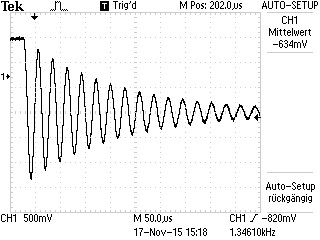
\includegraphics[width=\textwidth]{data/F0000TEK.jpg}
  \caption{Zeitlicher Spannungsverlauf des gedämpften Schwingkreises}
  \label{fig:5aergebnis}
\end{figure}
Abb. \ref{fig:5aergebnis} zeigt den Verlauf der Spannung in dem gedämpften
Schwingkreis. Gut zu erkennen sind die sinusförmige Schwingung und
die einhüllende e-Funktion, die die Dämpfung beschreibt.
Die Frequenz beträgt 1,35 kHz.
Die Extremstellen der Spannungen sind in Tabelle \ref{tab:5a} dargestellt,
für die übrigen, für die Auswertung weniger relevanten
Werte sei auf Quelle \cite{messwerte} verwiesen.
\begin{table}
\noindent
\centering
\caption{Extrema der Spannungen (Offset beachten))}
\label{tab:5a}
\sisetup{table-format=1.2}
\begin{tabular}{rr}
\toprule
{$t$ [\si{\milli\second}]} & {$U$[V]} \\
\midrule
-0.021 \pm 0.0005 & 0.78 \pm 0.005\\
-0.006 \pm 0.0005  & -2.06 \pm 0.005\\
0.008 \pm 0.0005 & 0.54 \pm 0.005\\
0.023 \pm 0.0005 & -1.88 \pm 0.005\\
0.037 \pm 0.0005 & 0.36 \pm 0.005\\
0.052 \pm 0.0005 & -1.70 \pm 0.005\\
0.066 \pm 0.0005 & 0.18 \pm 0.005\\
0.081 \pm 0.0005 & -1.56 \pm 0.005\\
0.095 \pm 0.0005 & 0.08 \pm 0.005\\
0.110 \pm 0.0005 & -1.44 \pm 0.005\\
0.125 \pm 0.0005 & -0.04 \pm 0.005\\
0.138 \pm 0.0005 & -1.34 \pm 0.005\\
0.152 \pm 0.0005 & -0.14 \pm 0.005\\
0.168 \pm 0.0005 & -1.24 \pm 0.005\\
0.182 \pm 0.0005 & -0.22 \pm 0.005\\
0.197 \pm 0.0005 & -1.18 \pm 0.005\\
0.210 \pm 0.0005 & -0.30 \pm 0.005\\
0.226 \pm 0.0005 & -1.12 \pm 0.005\\
0.239 \pm 0.0005 & -0.36 \pm 0.005\\
0.254 \pm 0.0005 & -1.06 \pm 0.005\\
0.268 \pm 0.0005 & -0.42 \pm 0.005\\
0.282 \pm 0.0005 & -1.02 \pm 0.005\\
\bottomrule
\end{tabular}
\end{table}

Der negative Zeitabschnitt bei den ersten beiden Messwerten
sowie die Tatsache, dass
die Messwerte der Spannung
offensichtlich einem Offset unterliegen,
spielt für die Berechnung des Dämpfungswiderstandes keine Rolle
(siehe Diskussion).
Als Spannungsamplitude wird im folgenden die Differenz zwischen Maximum und
Minimum der Spannung bezeichnet, auf Tabelle
\ref{tab:5a} bezogen also jeweils die
Differenz zweier aufeinanderfolgenden Werte.
Der Abfall der Spannung soll der Theorie
zufolge(siehe Gleichung \ref{eqn:Ischwingung})
mit $e^{-2\pi\mu t}$ erfolgen. Die Spannungsamplitude fällt bei t=\SI{0.0001816}
{\second} zum ersten Mal unter
$\frac{1}{e}$tel des ursprünglichen Wertes.
Da der erste Messwert
nicht bei t=0 aufgenommen wurde, ergibt sich also
\begin{equation}
T_\text{ex} = t_{1/e} - t_0 = \SI{0.182 +- 0.005}{\milli\second}
- \SI{-0.021+-0.005}{\milli\second}=\SI{0.203 +- 0.007}{\milli\second}.
\end{equation}
Der Exponent der e-Funktion muss zu diesem Zeitpunkt -1 betragen (auf 4$/e=e^-1$
abgefallen), es ergibt sich also:
\begin{equation}
  -2\pi\mu T_{ex} = -1 \\
  \implies \mu = \frac{1}{2\pi T_{ex}} =  \SI{784.0 +- 27.3}{\per\second}
\end{equation}
Damit ergibt sich für den effektiven Dämpfungswiderstand gemäß
Gleichung \ref{eqn:mu} -umgestellt nach $R$- zu $R_\text{eff}= \SI{99.6+-3.4}{\ohm}$
und damit \num{107+-0.7}\% höher als der Nennwdiderstand.
\subsection{Aperiodischer Grenzfall}
\begin{figure}
  \centering
  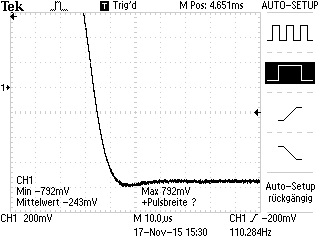
\includegraphics[width=\textwidth]{data/F0001TEK.jpg}
  \caption{Spannungsverlauf bei aperiodischer Dämpfung mit $R = \SI{3120 +- 20}{\ohm}$.}
  \label{fig:5bergebnis}
\end{figure}
Abb.\ref{fig:5bergebnis} zeigt den gemessenen Spannungsabfall für
$R = \SI{3120 +- 20}{\ohm}$.
Bei diesem Widerstand tritt die aperiodische Dämpfung auf, was daran zu erkennen
ist dass kein Überschwingen stattfindet wie z.B. in Abb.\ref{fig:über}, bei
der ein Widerstand von $R = \SI{2260 +- 20}{\ohm}$ eingestellt wurde.
\begin{figure}
  \centering
  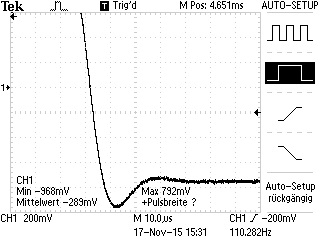
\includegraphics[width=\textwidth]{data/F0002TEK.jpg}
  \caption{Spannungsverlauf bei aperiodischer Dämpfung mit $R \neq R_{ap}$}
  \label{fig:über}
\end{figure}

Der theoretische Wert berechnet sich gemäß:
\begin{equation}
  \frac{1}{LC} = R_\text{ap}^2/4L^2 \\
  \implies R_\text{ap} = \sqrt{\frac{4L}{C}} = \SI{4390.4 \pm 9.0}{\ohm}.
\end{equation}

Für den Fehler gilt dabei gemäß der Gaußschen Fehlerfortpflanzung:
\begin{equation}
  \Delta R = \sqrt{\left.\frac{\partial L}{\partial R(C,L)}\right.\Delta L
  + \left.\frac{\partial R(C,L)}{\partial C}\right. \Delta C}
  \label{eqn:gauss}
\end{equation}

Der theoretische Wert weicht recht deutlich (\~30\%) von dem gemessenen ab.
Eine Erklärung dafür könnten die weiteren internen Widerstände sein, die in
der Schaltung in Form von Kabel u.ä. enthalten sind. Außerdem ist die Toleranz
des regelbaren Widerstandes nicht bekannt. Die Ungenauigkeit von R liegt also
tatsächlich höher als die angegeben \SI{+-20}{\ohm}.

\subsection{Resonanzüberhöhung}
\label{sec:5c}
Um die Resonanzüberhöhung zu bestimmen, wird zunächst die Kondensatorspannung
relativ zu der Erregerspannung berechnet. Da beide Werte mit dem selben Tastkopf
gemessen wurden, kann die Frequenzabhängigkeit dieses vernachlässigt werden
und man erhält $U_{rel}=\frac{U_c}{U_0}$. Die Messwerte sind in
Tabelle \ref{tab:5b} dargestellt.
\begin{table}[H]
\centering
\caption{Frequenzabhängige Spannung an Schwingkreis und Generator)}
\label{tab:5b}
\sisetup{table-format=1.2}
\begin{tabular}{lll}
\toprule
{$U_c$[V]} & {$U_0$[V]} &{$f$[kHz]}\\
\midrule
1.28 \pm 0.005 & 1.44 \pm 0.005 & 4.26 \pm 0.005\\
1.48 \pm 0.005 & 1.45 \pm 0.005 & 6.00 \pm 0.005\\
1.51 \pm 0.005 & 1.44 \pm 0.005 & 8.00 \pm 0.005\\
1.56 \pm 0.005 & 1.44 \pm 0.005 & 10.00 \pm 0.005\\
1.60 \pm 0.005 & 1.45 \pm 0.005 & 12.00 \pm 0.005\\
1.71 \pm 0.005 & 1.44 \pm 0.005 & 14.00 \pm 0.005\\
1.80 \pm 0.005 & 1.48 \pm 0.005 & 16.00 \pm 0.005\\
1.93 \pm 0.005 & 1.48 \pm 0.005 & 18.00 \pm 0.005\\
2.10 \pm 0.005 & 1.48 \pm 0.005 & 20.00 \pm 0.005\\
2.33 \pm 0.005 & 1.48 \pm 0.005 & 22.00 \pm 0.005\\
2.60 \pm 0.005 & 1.48 \pm 0.005 & 24.00 \pm 0.005\\
3.00 \pm 0.005 & 1.48 \pm 0.005 & 26.00 \pm 0.005\\
3.50 \pm 0.005 & 1.48 \pm 0.005 & 28.00 \pm 0.005\\
4.28 \pm 0.005 & 1.52 \pm 0.005 & 30.00 \pm 0.005\\
4.96 \pm 0.005 & 1.48 \pm 0.005 & 32.00 \pm 0.005\\
5.52 \pm 0.005 & 1.38 \pm 0.005 & 34.00 \pm 0.005\\
4.92 \pm 0.005 & 1.38 \pm 0.005 & 36.00 \pm 0.005\\
4.08 \pm 0.005 & 1.44 \pm 0.005 & 38.00 \pm 0.005\\
3.20 \pm 0.005 & 1.48 \pm 0.005 & 40.00 \pm 0.005\\
\bottomrule
\end{tabular}
\end{table}
\begin{figure}[H]
  \centering
  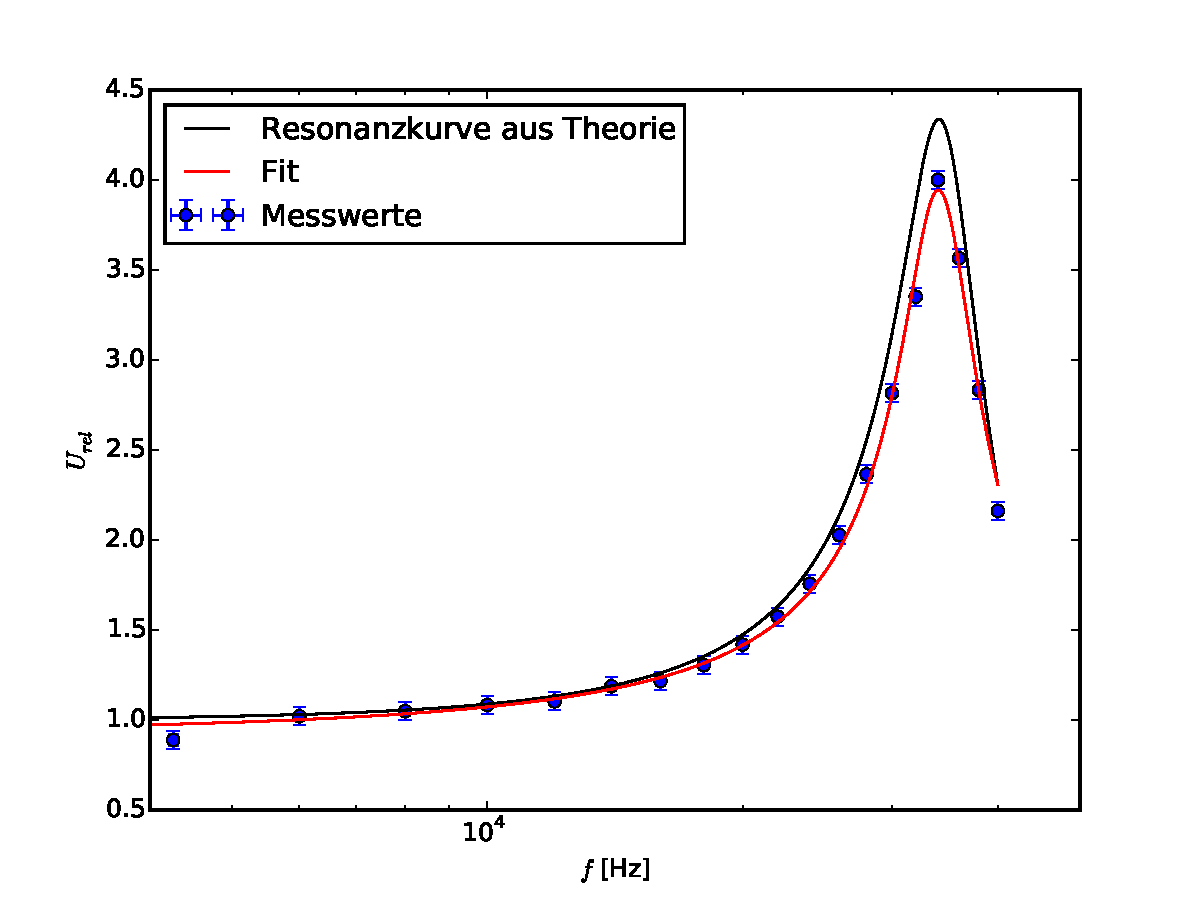
\includegraphics[width=\textwidth]{5cfit.pdf}
  \caption{Halblogarithmische Auftragung von $U_\text{rel}$ gegen $f$}
  \label{fig:5cergebnis}
\end{figure}
In Abb.\ref{fig:5cergebnis} lässt sich das qualitativ erwartete Ergebnis
wiederfinden. Um die Resonanzfrequenz $\omega_0$ steigt die Kondensatorspannung
sprunghaft an, für geringe Frequenzen nähert sie sich der Erregerspannung $U_0$
($\rightarrow U_{rel}=1$). Die in der Abbildung aufgetragene Resonanzkurve
deckt sich in weiten Teilen mit den Messwerten. Um die Resonanzfrequenz verläuft
die Resonanzkurve etwas höher.

Auffällig ist der Messert bei $f$=\SI{4.26}{\kilo\hertz},
bei dem die Kondensatorspannung unter
$U_0$ fällt. Dies ist mit der Theorie nicht vereinbar und am ehesten auf einen
Fehler bei der Messung von $U_c$ zurückzuführen. Die maximale Spannung liegt
bei $U_{max} = \SI{5.52 +- 0.005}{\volt}$. $U_0$ beträgt dabei \SI{1.38 +- 0.005}
{\volt}, damit beträgt die Resonanzüberhöhung \num{4.000 +- 0.015}.

Zur Bestimmung der Schärfe der Resonanz ist es zweckmäßig den Bereich um die
Resonanzfrequenz linear darzustellen, so zu sehen in Abb.\ref{fig:5clin}.
\begin{figure}[H]
  \centering
  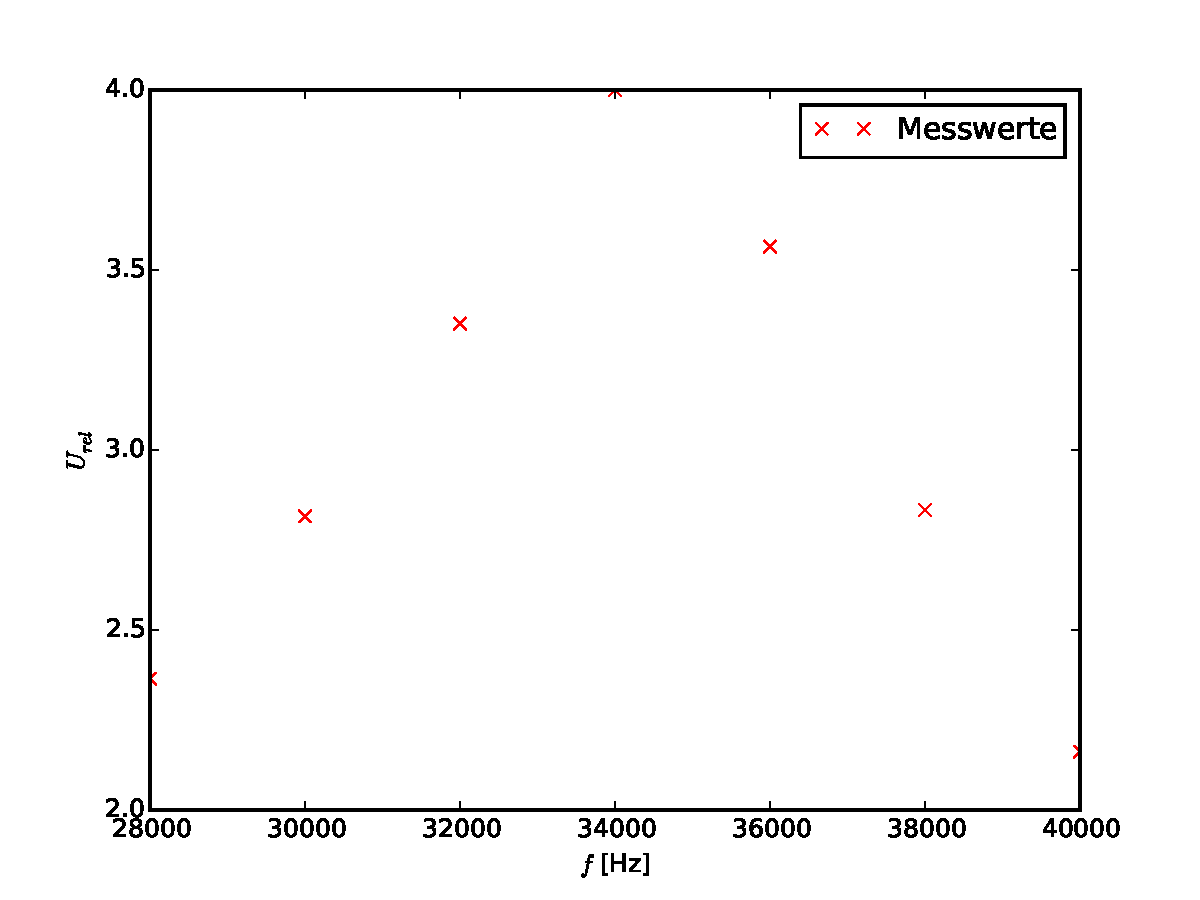
\includegraphics[width=\textwidth]{5c2.pdf}
  \caption{$U_{rel}$ um die Resonanzfrequenz linear aufgetragen}
  \label{fig:5clin}
\end{figure}
Die Resonanzfrequenz liegt im Rahmen der aufgenommenen Messwerte bei
$\omega$ = \SI{34 +- 1}{\kilo\hertz}.
In vorliegendem Fall entspricht $U_{rel}(\omega_{\pm})$ dem 2.83 fachen von $U_0$.
Diese Werte werden bei $\omega_-$ = \SI{30+-1}{\kilo\hertz}
($U_{rel}=\num{2.816+-0.01}$) und
$\omega_+$=\SI{38+-1}{\kilo\hertz} ($U_{rel} = \num{2.833+-0.01}$)
(Vgl. Tabelle \ref{tab:5b}) erreicht.
Gemäß Gleichung \ref{eqn:güte2} ergibt
sich demnach für die Güte:

$$q = \frac{\SI{34+-1}{\kilo\hertz}}{\SI{38+-1}{\kilo\hertz}-\SI{30+-1}
{\kilo\hertz}} = \num{4.2+-0.8}$$ .

Dieser Wert weicht nur um \num{6.0+-0.17}\% von dem Wert ab, der aus der maximalen
Spannung hergeleitet wurde. Die Abweichung lässt sich neben Messfehlern in erster
Linie auf die geringe Anzahl an Messwerten im Bereich der Resonanzfrequenz
zurückführen. Dadurch ist die Genauigkeit bei der Bestimmung von
$U_{Cmax}$ sowie $\omega_\pm$ begrenzt. Die maximale Spannung kann durchaus
einige Prozentpunkte höher als der höchste gemessene Wert von $4\cdot U_0$
liegen.
Berechnet man die Güte anhand der Parameter des Schwingkreises
(Vgl. Gleichung \ref{eqn:güte1}) erhält man mit: \\
$L = \SI{10.11 +- 0.03}{\milli\henry}$  \\
$C = \SI{2.098 +- 0.006}{\nano\farad}$ und \\
$R = \SI{509.5 +- 0.5}{\ohm}$ \\
für die Güte:

$q = 4.309 \pm 0.010$.

Dieser Wert liegt in guter Übereinstimmung mit den beiden aus den Messwerten
erhaltenen Werten für q.

\subsection{Phasenverschiebung}
Die Messwerte für $\phi$ sind in folgender Tabelle auffgelistet, Abb.
\ref{fig:5dlog} zeigt $\phi$ in Abhängigkeit von der Frequenz $f$ mit
logarithmischer x-Achse, Abb.\ref{fig:5dlin} den Bereich um $\phi$ = 90° mit
linearen Achsenskalierungen.
Bei dem Vergleich der Messwerte mit der Theoriekurve in Abb.\ref{fig:5dlog}
fällt auf, dass die Messwerte nicht wie zu erwarten durch $\frac{\pi}{2}$
beschränkt sind (siehe Diskussion).
\begin{table}
\centering
\caption{Phasenverschiebung in Abhängigkeit von der Frequenz)}
\label{tab:5c}
\sisetup{table-format=1.2}
\begin{tabular}{rr}
\toprule
{$\phi$[deg]} &{$f$[kHz]}\\
\midrule
7.67\pm 0.005 & 4.26\pm 0.005 \\
6.48\pm 0.005 & 6.00\pm 0.005 \\
3.46\pm 0.005 & 8.00\pm 0.005 \\
1.44\pm 0.005 & 10.00\pm 0.005 \\
5.18\pm 0.005 & 12.00\pm 0.005 \\
6.05\pm 0.005 & 14.00\pm 0.005 \\
10.37\pm 0.005 & 16.00\pm 0.005 \\
12.96\pm 0.005 & 18.00\pm 0.005 \\
11.52\pm 0.005 & 20.00\pm 0.005 \\
19.01\pm 0.005 & 22.00\pm 0.005 \\
17.28\pm 0.005 & 24.00\pm 0.005 \\
22.46\pm 0.005 & 26.00\pm 0.005 \\
32.26\pm 0.005 & 28.00\pm 0.005 \\
45.36\pm 0.005 & 30.00\pm 0.005 \\
57.60\pm 0.005 & 32.00\pm 0.005 \\
80.78\pm 0.005 & 34.00\pm 0.005\\
108.86\pm 0.005 & 36.00\pm 0.005 \\
125.86\pm 0.005 & 38.00\pm 0.005 \\
141.12\pm 0.005 & 40.00\pm 0.005 \\
\bottomrule
\end{tabular}
\end{table}

\begin{figure}
  \centering
  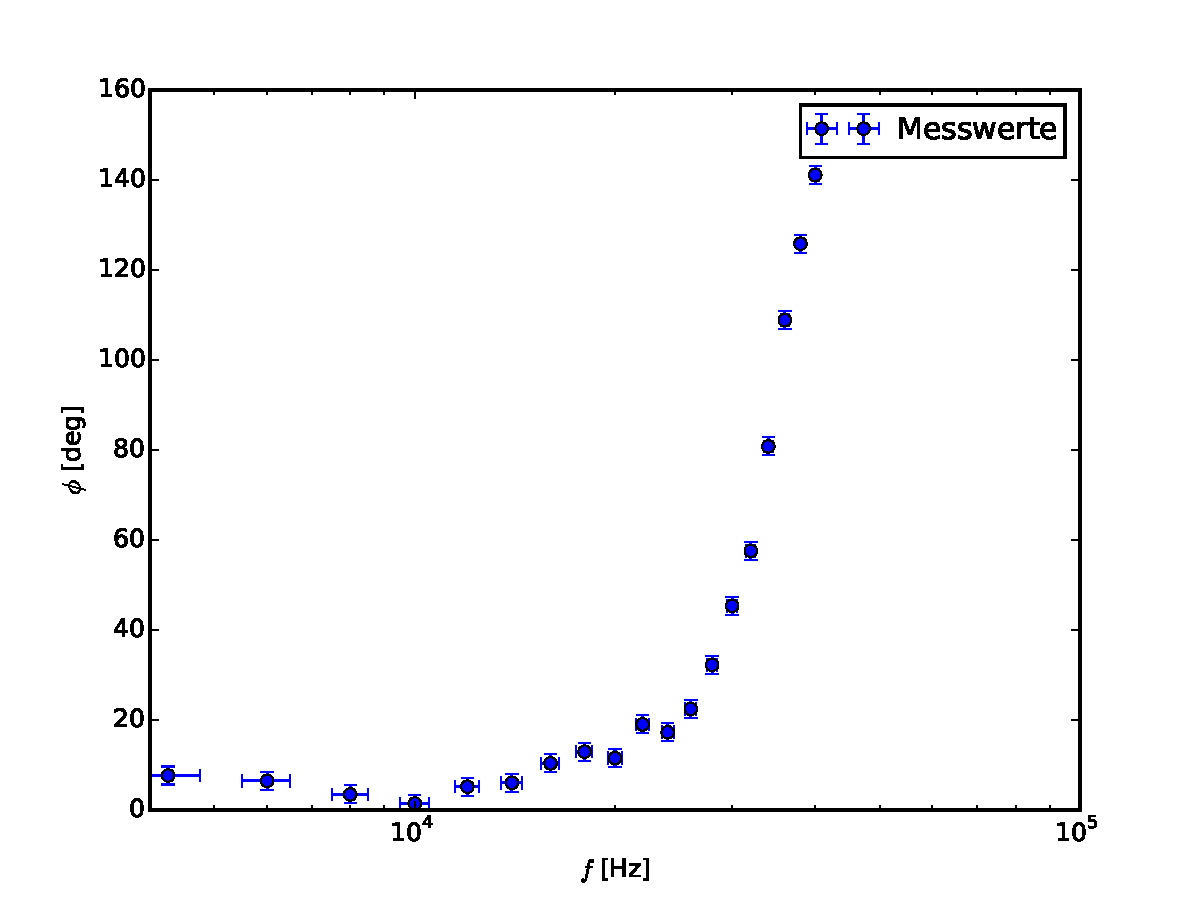
\includegraphics[width=\textwidth]{5d.pdf}
  \caption{Phasenverschiebung $\phi$ mit logarithmischer x-Achsenskalierung}
  \label{fig:5dlog}
\end{figure}

\begin{figure}
  \centering
  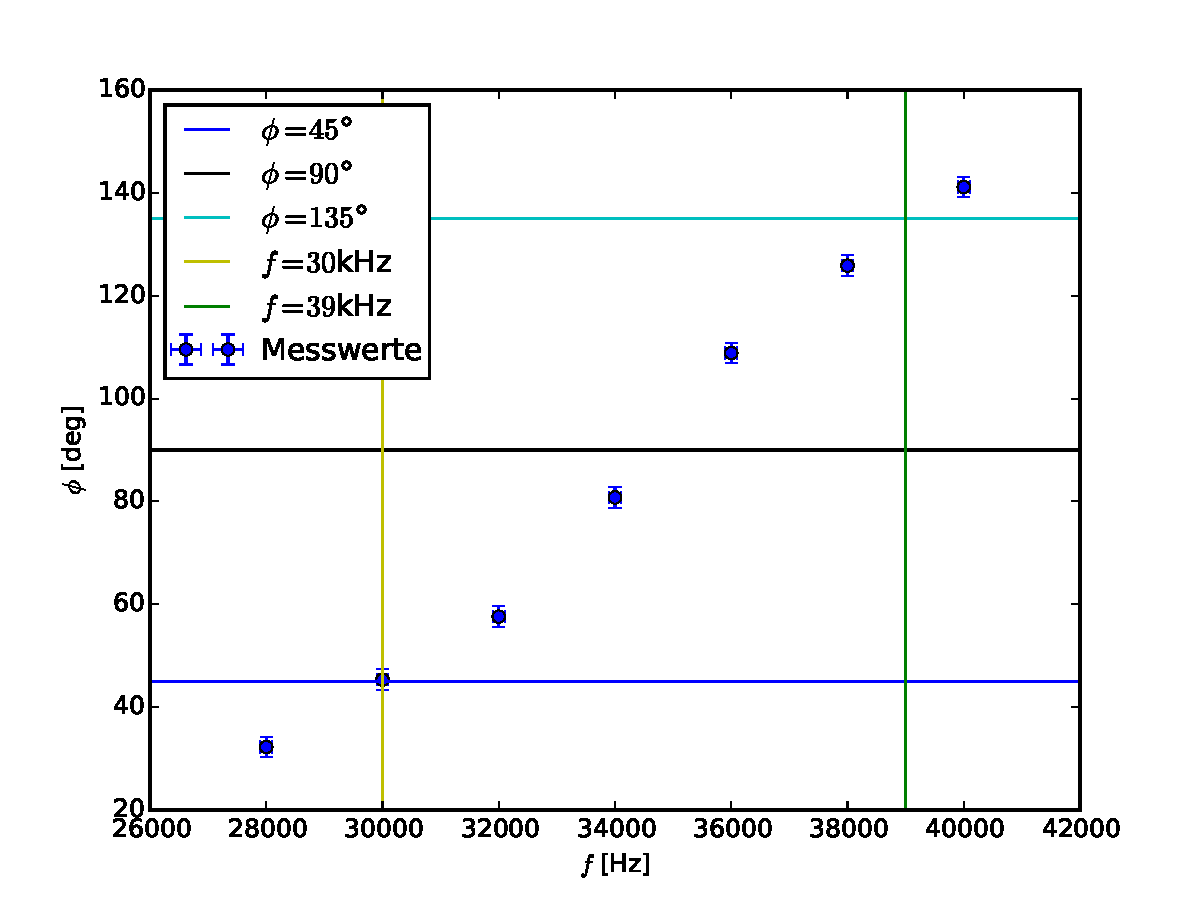
\includegraphics[width=\textwidth]{5d2.pdf}
  \caption{Phasenverschiebung $\phi$ im Bereich der Resonanzfrequenz mit
  linearer Achsenskalierung}
  \label{fig:5dlin}
\end{figure}

In Abb. \ref{fig:5dlin} sind außerdem die Geraden eingetragen um das Ablesen
der relevanten Phasenverschiebungen zu erleichtern.
$\omega_1$ ($\phi$ = 45°) liegt ziemlich fast exakt bei 30kHz ($\phi$=45,36°),
$\omega_2$ liegt bei \~ 39kHz. Damit liegen $\omega_1$ und $\omega_2$ bei
ähnlichen Frequenzen wie zuvor (Vgl. Abschnitt \ref{sec:5c}) schon $\omega_-$
und $\omega_+$ Dies ist das erwartete Ergebnis für den Fall schwacher
Dämpfung, der hier realisiert ist. $\omega_1$ und $\omega_-$ sind im Rahmen
der begrenzten Anzahl an Messwerten identisch, $\omega_2$ und $\omega_+$ weichen
um \~13\% voneinander ab.
